\section{Systemdesign}

\subsection{Språk}
Programmet som skall lösa optimeringsproblemmet kommer att skrivas i programmeringsspråket C. 

\subsection{Standarder}
Källkoden kommer följa de standarder som är beskrivna i kvalitetsplanen.

\subsection{Systemskiss}
Programmet kommer i huvudsak köras via matlab, där programmet kommer anropas som en funktion med all indata i parametrarna. Indatan kommer sedan kompileras till en header fil som sedan skickas till solvern. QP-solvern kommer sedan lösa problemet utifrån kompilerade datan och sedan returnera resultatet till matlab.

% Graphic for TeX using PGF
% Title: C:\Users\sebfas\Pictures\Systemskiss.dia
% Creator: Dia v0.97.2
% CreationDate: Sun Feb 15 00:30:41 2015
% For: sebfas
% \usepackage{tikz}
% The following commands are not supported in PSTricks at present
% We define them conditionally, so when they are implemented,
% this pgf file will use them.
\ifx\du\undefined
  \newlength{\du}
\fi
\setlength{\du}{15\unitlength}
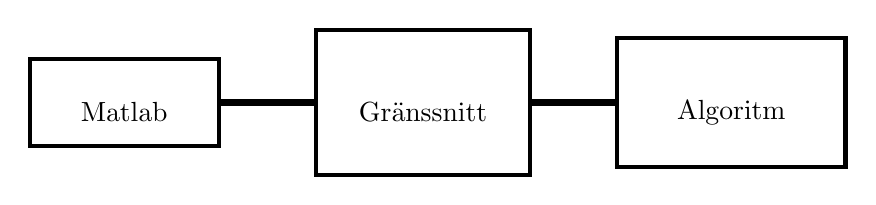
\begin{tikzpicture}
\pgftransformxscale{1.000000}
\pgftransformyscale{-1.000000}
\definecolor{dialinecolor}{rgb}{0.000000, 0.000000, 0.000000}
\pgfsetstrokecolor{dialinecolor}
\definecolor{dialinecolor}{rgb}{1.000000, 1.000000, 1.000000}
\pgfsetfillcolor{dialinecolor}
\definecolor{dialinecolor}{rgb}{1.000000, 1.000000, 1.000000}
\pgfsetfillcolor{dialinecolor}
\fill (1.400000\du,1.700000\du)--(1.400000\du,3.800000\du)--(5.950000\du,3.800000\du)--(5.950000\du,1.700000\du)--cycle;
\pgfsetlinewidth{0.100000\du}
\pgfsetdash{}{0pt}
\pgfsetdash{}{0pt}
\pgfsetmiterjoin
\definecolor{dialinecolor}{rgb}{0.000000, 0.000000, 0.000000}
\pgfsetstrokecolor{dialinecolor}
\draw (1.400000\du,1.700000\du)--(1.400000\du,3.800000\du)--(5.950000\du,3.800000\du)--(5.950000\du,1.700000\du)--cycle;
% setfont left to latex
\definecolor{dialinecolor}{rgb}{0.000000, 0.000000, 0.000000}
\pgfsetstrokecolor{dialinecolor}
\node at (3.675000\du,2.990000\du){Matlab};
\definecolor{dialinecolor}{rgb}{1.000000, 1.000000, 1.000000}
\pgfsetfillcolor{dialinecolor}
\fill (8.300000\du,1.000000\du)--(8.300000\du,4.500000\du)--(13.450000\du,4.500000\du)--(13.450000\du,1.000000\du)--cycle;
\pgfsetlinewidth{0.100000\du}
\pgfsetdash{}{0pt}
\pgfsetdash{}{0pt}
\pgfsetmiterjoin
\definecolor{dialinecolor}{rgb}{0.000000, 0.000000, 0.000000}
\pgfsetstrokecolor{dialinecolor}
\draw (8.300000\du,1.000000\du)--(8.300000\du,4.500000\du)--(13.450000\du,4.500000\du)--(13.450000\du,1.000000\du)--cycle;
% setfont left to latex
\definecolor{dialinecolor}{rgb}{0.000000, 0.000000, 0.000000}
\pgfsetstrokecolor{dialinecolor}
\node at (10.875000\du,2.990000\du){Gränssnitt};
\definecolor{dialinecolor}{rgb}{1.000000, 1.000000, 1.000000}
\pgfsetfillcolor{dialinecolor}
\fill (15.550000\du,1.200000\du)--(15.550000\du,4.300000\du)--(21.050000\du,4.300000\du)--(21.050000\du,1.200000\du)--cycle;
\pgfsetlinewidth{0.100000\du}
\pgfsetdash{}{0pt}
\pgfsetdash{}{0pt}
\pgfsetmiterjoin
\definecolor{dialinecolor}{rgb}{0.000000, 0.000000, 0.000000}
\pgfsetstrokecolor{dialinecolor}
\draw (15.550000\du,1.200000\du)--(15.550000\du,4.300000\du)--(21.050000\du,4.300000\du)--(21.050000\du,1.200000\du)--cycle;
% setfont left to latex
\definecolor{dialinecolor}{rgb}{0.000000, 0.000000, 0.000000}
\pgfsetstrokecolor{dialinecolor}
\node at (18.300000\du,2.990000\du){Algoritm};
\pgfsetlinewidth{0.150000\du}
\pgfsetdash{}{0pt}
\pgfsetdash{}{0pt}
\pgfsetbuttcap
{
\definecolor{dialinecolor}{rgb}{0.000000, 0.000000, 0.000000}
\pgfsetfillcolor{dialinecolor}
% was here!!!
\definecolor{dialinecolor}{rgb}{0.000000, 0.000000, 0.000000}
\pgfsetstrokecolor{dialinecolor}
\draw (5.950000\du,2.750000\du)--(8.300000\du,2.750000\du);
}
\pgfsetlinewidth{0.150000\du}
\pgfsetdash{}{0pt}
\pgfsetdash{}{0pt}
\pgfsetbuttcap
{
\definecolor{dialinecolor}{rgb}{0.000000, 0.000000, 0.000000}
\pgfsetfillcolor{dialinecolor}
% was here!!!
\definecolor{dialinecolor}{rgb}{0.000000, 0.000000, 0.000000}
\pgfsetstrokecolor{dialinecolor}
\draw (13.450000\du,2.750000\du)--(15.550000\du,2.750000\du);
}
\end{tikzpicture}


\subsection{Syfte}
Syftet med arkitekturen är att skapa en översikt av hela systemet för att man på ett enkelt sätt ska få en överblick av hur alla moduler hänger ihop och hur de fungerar. Den är även ett underlag för att kunna skapa den slutgiltliga tekniska dokumentationen.

\subsection{Prestanda}
Det är av yttersta vikt att programmet löser QP-problemet väldigt snabbt, i samma skala som Gurobi. Detta är dels för att flygplanet ska hinna utföra prediktionsregleringen i tid.

\subsection{Stabilitet}
Programmet måste kunna klara av
